\documentclass{article}
\usepackage{a4wide}
\usepackage{amssymb}
\usepackage{amsmath}
\usepackage[numbers]{natbib}
\usepackage{xcolor}
\usepackage[colorlinks,linkcolor=blue,urlcolor=blue,citecolor=blue]{hyperref}
\usepackage{mathrsfs}
\usepackage{comment}
\usepackage{tabularx}
\usepackage{booktabs}
\usepackage{caption}% http://ctan.org/pkg/caption
\captionsetup[table]{justification=raggedright, singlelinecheck=off}
\usepackage{amsthm}
\theoremstyle{definition}
\usepackage{pgf}
\usepackage{tikz}
\usetikzlibrary{arrows,automata}

\usepackage{tikz}
\usetikzlibrary{calc,positioning,shapes,arrows,decorations.pathreplacing}
\usetikzlibrary{shapes.multipart}


\title{Resource Constrained Project Scheduling for continuous applications using Precedence Constraint Posting.}
\author{M. van Gelderen  \and
    R.M. de Lange \and
    B. Gris\`el \and
    F. van Tienen}
\date{}

\pagestyle{empty}

\newcommand{\TODO}[1]{{\color{red}\textbf{TODO: #1}}}
\newtheorem{example}{Example}[section]

\newcommand{\res}[0]{\ensuremath{R}} %resources
\newcommand{\av}[1]{\ensuremath{av(r_{#1})}} %availability
\newcommand{\capa}[1]{\ensuremath{cap(r_{#1})}} %capacity
\newcommand{\dur}[1]{\ensuremath{dur(v_{#1})}} %durability
\newcommand{\usage}[2]{\ensuremath{usage(v_{#1}, r_{#2})}} %usage of resource #2 by activity #1
\newcommand{\start}[1]{\ensuremath{start(v_{#1})}} %start time
\newcommand{\makespan}[1]{\ensuremath{C_{max}(#1)}} %makespan

\newenvironment{definition}[1][Definition]{\begin{trivlist}
\item[\hskip \labelsep {\bfseries #1}]}{\end{trivlist}}

\setlength{\parindent}{0pt}
\setlength{\parskip}{\baselineskip}

\begin{document}
\maketitle
\thispagestyle{empty}

\begin{abstract}
\TODO{rewrite when paper finished}
\end{abstract}


\newpage


\section{Scope and purpose}

In this paper we will discus the resource constraint scheduling problem in practical applications.
Scheduling is a very common problem in many day-to-day applications, because many situations require a suitable schedule to define the order in which to perform different tasks.
Making a schedule proves to be a more complex process than one might expect, especially when complicating factors arise such as limited resources or a set deadline.
These factors can be taken into account to some extent by the resource constraint scheduling problem.
Some other complicating factors may occur in practical applications, such as the possibility of break down of resources, delays or a growing set of tasks.
The scheduling problem is therefore, although it is quite common, one of the more complex problems in computer science.

This paper will deal with the scheduling problem, some complicating factors and the solution to this problem in continuous applications.
Because of its common usage in practical applications and the complexity of the problem, the way the solution is approximated gives an interesting insight in the problem.
In almost all practical application, an approximation is used to retrieve a schedule.
Although these approximations do not deliver the optimal solution to a problem, they often give a good working schedule in less time than an optimal solution.
For a continuous environment, this quick solution is key to keep up with the constant changes.

An approximation method will be discussed in light of the practical applications of the scheduling problem.
For the approximation simple temporal networks will be used, these allow to give a more simple representation of the complex scheduling problem.
Simple temporal networks are a form of graph representations using the nodes and edges to represent the tasks, resources and constraints in the original scheduling problem.
One must note that this simpler representation does not allow for all scheduling problems to be represented correctly, therefore some solutions which are in fact feasible, might not be found using the approximation.

The purpose of this paper is to inform the reader on the topic of resource constraint scheduling in continuous applications.
The paper aims to be a good source of information on the topic of resource constraint scheduling and its link to the practical applications seen in daily life.
Although the reader is presumed to have prerequisite knowledge about for example set theory, graph theory, algorithmics and complexity theory, most in-depth information aims to be complete and clear.

%		-Wat staat waar?
In the chapter \emph{Problem Background} \ref{text:problem_background} we will first go deeper in to the resource constraint scheduling problem.
Here the different aspects of the resource constraint scheduling problem will be discussed.
An example of a scheduling problem will be given, along with an intuitive description and formal definitions of the problem.
We will also look into the complexity \ref{text:complex} \TODO{ref} of the problem, showing why an approximation is needed for practical applications.

The following chapter, \emph{Schedule Construction} \ref{text:schedule} \TODO{ref}, will deal with the approximation of the solution.
For the approximation, simple temporal networks \ref{text:STN} \TODO{ref} will be used, which provide with a simpler way of representing a schedule.
The simple temporal networks will be explained using the example from the previous chapter and again giving an intuitive and formal definition.
When a more dynamic way of adapting the schedule is required, precedence constraint posting \ref{text:PCP} \TODO{ref} is introduced to the simple temporal networks.
Precedence constraint posting is a technique which allows for changes to a temporal network by introducing new precedence constraints.
The workings of precedence constraint posting will also be explained using the example and giving an intuitive and formal definition.

Combining these two methods gives us a flexible way of approximating a resource constraint scheduling problem.
Concluding we will show that this combination provides us with a solution capable of scheduling complex problems in continuous environments.
This gives us a robust and effective solution for scheduling in many practical applications.


\newpage


\section{Problem background}
\label{text:problem_background}

\TODO{Roelf: intro}
%		-What are scheduling problems?
%		-Examples form real life.
%		-What is RSPCP and how can it solve them.
%		-Why imporant.
%		-Voorbeelden wat meer uitwerken. Intuitief verhaal.}

\TODO{Freek: running example}

\subsection{Running example}
In this paper we will use a simple running example based on a painting job to explain the RCPSP.

The problem consists of workers that need to finish three painting jobs: a door, a fence and a wall.
Because the the door and the fence are made of wood, both surfaces needs to be sanded first (\emph{precedence constraints}).
Sanding is not necessary for the wall, because the wall is made of bricks.
When the job is finished all painting brushes need to be cleaned and this can only be done when all the painting is finished.
This gives us six \emph{activities}: sanding the the door, sanding the fence,  painting the door, painting the fence, painting the wall and cleaning the painting brushes.
And the following precedence constraints: sanding the door before painting the door, sanding the fence before painting the fence and all the painting activities need to be done before cleaning the painting brushes.

Because the size of each surface in the painting jobs differs, not each activity takes the same amount of time to finish (\emph{duration}).
Since this is not the first painting job the workers have done, we assume that they know the exact duration for each activity:
\begin{itemize}
\item sanding the door: 3 hours
\item sanding the fence: 2 hours
\item painting the door: 2 hours
\item painting the fence: 1 hour
\item painting the wall: 5 hours
\item cleaning the painting brushes: 1 hour
\end{itemize}
% moet nog even goed gestyled worden en even gecontroleerd worden of tijden beetje goed zijn
Normally this would be an easy job, but they have forgotten a lot of their tools (\emph{resources}).
So now they only have two painting brushes and one sanding machine (\emph{resource constraints}), which makes it impossible to sand more than one surface at the same time and to paint more than two surfaces at the same time.
This shows us that the \emph{capacity} of painting surfaces at the same time is two and the capacity of sanding surfaces at the same time is one.

Since every sanding job uses the sanding machine as a resource, the usage of sanding the door and sanding the fence is $1$ for the sanding machine.
Also every painting job uses the painting brush as a resource, so that painting the door, painting the fence and painting the wall all have a usage of $1$ on the painting brush.
There is only one activity left, cleaning the painting brushes, which will use both of the painting brushes resource so that the usage on the painting brushes is $2$.
Because a sanding activity doesn't use a painting brush, a painting activity doesn't use a sanding machine and cleaning the painting brushes doesn't use a sanding machine all of the other usages are $0$.

The painters want to make a schedule, where they define each starting time for the activities in such a way that the resulting schedule is feasible.
This means that the sanding of each wooden surface (the door and the wall) needs to be finished before starting the painting of that surface.
Because of the limited resources, they can never paint more than two surfaces at the same time, or sand more than one surface at the same time.
There are also a lot of other jobs to do, so the painter not only want a feasible schedule but also want to optimize the time in which they finish all the activities.

\subsection{Definition}

\begin{figure}[h]
	\centering
	% Author: Mick van Gelderen
% Created from http://www.texample.net/tikz/examples/class-diagram/ and other examples and resources. 

%\documentclass{standalone}
%\usepackage{tikz}
\usetikzlibrary{calc,positioning,shapes,arrows,decorations.pathreplacing}
\usetikzlibrary{shapes.multipart}


%\begin{document}

\tikzstyle{activity}=[rectangle, draw=black, text centered, text=black, thick, minimum height=1.8em, minimum width=1.8em]
\tikzstyle{dummy}=[rectangle, fill=black!7, draw=black, text centered, text=black, thick, minimum height=1.8em, minimum width=1.8em]
\tikzstyle{precedence}=[->,>=stealth, draw=black!70, thick]

\newcommand{\activity}[3]{\node (v#1) [activity, text width=#2cm, #3] {$v_#1$};}

\begin{tikzpicture}[node distance=.8cm]
		\node (v0) [dummy] {$v_0$};
    \activity{2}{2}{right=1.6cm of v0}
    \activity{1}{3}{above=of v2}
    \activity{3}{2}{right=of v1}
    \activity{4}{1}{below=of v3}
    \activity{5}{5}{below=of v2}
    \activity{6}{1}{right=1.6cm of v4}
		\node (v7) [dummy, right=of v6] {$v_7$};
		
    \draw[precedence] (v0.east) to[out=0,in=180] (v1.west);
    \draw[precedence] (v0.east) to[out=0,in=180] (v2.west);
    \draw[precedence] (v0.east) to[out=0,in=180] (v5.west);
    \draw[precedence] (v1.east) to[out=0,in=180] (v3.west);
    \draw[precedence] (v2.east) to[out=0,in=180] (v4.west);
    \draw[precedence] (v3.east) to[out=0,in=180] (v6.west);
    \draw[precedence] (v4.east) to[out=0,in=180] (v6.west);
    % start bending from the projection v4 on the line y=v3.y
    \draw[precedence] (v5.east) -- ($(v5)!(v4)!($(v5)+(1,0)$)$) to[out=0,in=180] (v6.west);
		\draw[precedence] (v6.east) to[out=0,in=180] (v7.west);		    

    % Descriptions
    \path (v3.east) to[out=0,in=180] coordinate (temp) (v6.west);
    \draw[shorten <=2pt, shorten >=2pt] (temp) -- ++(.8,.6) node[anchor=west, yshift=2pt, text width=2cm] {Precedence constraint $(v_3, v_6) \in E$};
    
    \draw[shorten <=2pt, shorten >=2pt] (v5.south) -- ++(.8,-.6) node[anchor=west, yshift=-2pt] {Activity $v_5$};
    
    % Funky braces
    \draw[decorate,decoration={brace,amplitude=8pt}]
        let \p1 = (v5.west), \p2 = (v6.east), \p3 = (v1) in 
        (\x1, \y3+1cm) -- (\x2, \y3+1cm) node[midway, above=10pt] {$V = \{v_1, \ldots, v_6\}$};
        
    \draw[decorate,decoration={brace,amplitude=8pt}]
        let \p1 = (v0.west), \p2 = (v7.east), \p3 = (v1) in 
        (\x1, \y3+2cm) -- (\x2, \y3+2cm) node[midway, above=10pt] {$W = V \cup \{v_0, v_7\}$};
    
\end{tikzpicture}

%\end{document}
	\caption{The activity graph for the running example. }
	\label{fig:activity_graph}
\end{figure}

\emph{Activities} are specified by a set $V = \{v_1, \ldots, v_n\}$.
This is a set of activities where the total amount of activities is $n \in \mathbb{N}$ and each activity is represented by a unique identifier. %identifier??
In the running example we have six activities ($n = 6$): sanding the the door $v_1$, sanding the fence $v_2$,  painting the door $v_3$, painting the fence $v_4$, painting the wall $v_5$ and cleaning the painting brushes $v_6$.
Which gives us the total set of activities $V = \{v_1, \ldots, v_6\}$ for the running example.
These activities are represented in Figure \ref{fig:activity_graph} as blocks.

The \emph{duration} for each activity $v_i \in V$ is specified by $\dur{i} \in \mathbb{N}$.
In the running example the activities have the following duration: $\dur{1} = 3, \dur{2} = 2, \dur{3} = 2, \dur{4} = 1, \dur{5} = 5, \dur{6} = 1$.
The duration of each activity in the running example is represented by the length of the block in Figure \ref{fig:activity_graph}.

\emph{Precedence constraints} are specified by a set $E = \{(v_i, v_j) | v_i \in V, v_j \in V, v_i \neq v_j\}$.
This means that a precedence relation between activities $v_i$ and $v_j$, where $v_j$ can be started only after $v_i$ is finished, is represented as $(v_i, v_j) \in E$.
The running example has several precedence constraints between the activities, which will give the following set $E = \{(v_1, v_3), (v_2, v_4), (v_3, v_6), (v_4, v_6), (v_5, v_6)\}$.
Figure \ref{fig:activity_graph} shows the precedence constraints for the running example, represented as arrows between the nodes.

The \emph{extended activity set} is specified by $W = V \cup \{v_0, v_{n+1}\}$.
Which consists of the activity set $V$ and incorporates a unique dummy beginning activity $v_0$ and a unique dummy ending activity $v_{n+1}$. 
These dummy activities have a duration of $0$ periods.
Precedence constraints are added to ensure that the starting activity starts before every other activity and that every activity is completed before the ending activity. 
For the running example we will have a set $W = \{v_0, \ldots v_7\}$.
Figure \ref{fig:activity_graph} shows $W$ for the running example. 

The \emph{constraints graph} is specified by a directed graph $G = (V, E)$.
It consists of the activities $V$, which are represented as nodes, and the precedence constraints $E$, which are represented as connections between nodes.
The constraints graph for the running example is represented in Figure \ref{fig:activity_graph}, where the precedence constraints are reduced to a minimum.

\begin{figure}[h]
	\centering
	% Author: Mick van Gelderen
% Created from http://www.texample.net/tikz/examples/class-diagram/ and other examples and resources. 

%\documentclass{standalone}
%\usepackage{tikz}
\usetikzlibrary{calc,positioning,shapes,arrows,decorations.pathreplacing}
\usetikzlibrary{shapes.multipart}


%\begin{document}

\tikzstyle{activity}=[rectangle, draw=black, text centered, text=black, thick, minimum height=1.8em, minimum width=1.8em]
\tikzstyle{dummy}=[rectangle, fill=black!7, draw=black, text centered, text=black, thick, minimum height=1.8em, minimum width=1.8em]
\tikzstyle{precedence}=[->,>=stealth, draw=black!70, thick]

\newcommand{\activity}[3]{\node (v#1) [activity, text width=#2cm, #3] {$v_#1$};}

\begin{tikzpicture}[node distance=.8cm]
		\node (v0) [dummy] {$v_0$};
    \activity{2}{2}{right=1.6cm of v0}
    \activity{1}{3}{above=of v2}
    \activity{3}{2}{right=of v1}
    \activity{4}{1}{below=of v3}
    \activity{5}{5}{below=of v2}
    \activity{6}{1}{right=1.6cm of v4}
		\node (v7) [dummy, right=of v6] {$v_7$};
		
    \draw[precedence] (v0.east) to[out=0,in=180] (v1.west);
    \draw[precedence] (v0.east) to[out=0,in=180] (v2.west);
    \draw[precedence] (v0.east) to[out=0,in=180] (v5.west);
    \draw[precedence] (v1.east) to[out=0,in=180] (v3.west);
    \draw[precedence] (v2.east) to[out=0,in=180] (v4.west);
    \draw[precedence] (v3.east) to[out=0,in=180] (v6.west);
    \draw[precedence] (v4.east) to[out=0,in=180] (v6.west);
    % start bending from the projection v4 on the line y=v3.y
    \draw[precedence] (v5.east) -- ($(v5)!(v4)!($(v5)+(1,0)$)$) to[out=0,in=180] (v6.west);
		\draw[precedence] (v6.east) to[out=0,in=180] (v7.west);		    

    % Descriptions
    \path (v3.east) to[out=0,in=180] coordinate (temp) (v6.west);
    \draw[shorten <=2pt, shorten >=2pt] (temp) -- ++(.8,.6) node[anchor=west, yshift=2pt, text width=2cm] {Precedence constraint $(v_3, v_6) \in E$};
    
    \draw[shorten <=2pt, shorten >=2pt] (v5.south) -- ++(.8,-.6) node[anchor=west, yshift=-2pt] {Activity $v_5$};
    
    % Funky braces
    \draw[decorate,decoration={brace,amplitude=8pt}]
        let \p1 = (v5.west), \p2 = (v6.east), \p3 = (v1) in 
        (\x1, \y3+1cm) -- (\x2, \y3+1cm) node[midway, above=10pt] {$V = \{v_1, \ldots, v_6\}$};
        
    \draw[decorate,decoration={brace,amplitude=8pt}]
        let \p1 = (v0.west), \p2 = (v7.east), \p3 = (v1) in 
        (\x1, \y3+2cm) -- (\x2, \y3+2cm) node[midway, above=10pt] {$W = V \cup \{v_0, v_7\}$};
    
\end{tikzpicture}

%\end{document}
	\caption{The resource relations for the running example. }
	\label{fig:resource_graph}
\end{figure}

\emph{Resources} are specified by a set $R = \{r_1, \ldots, r_m\}$.
The total amount of resources is $m \in \mathbb{N}$ and each resource is represented by a unique identifier. %identifier??
In the running example we have two resources ($m = 2$): the sanding machine $r_1$ and the painting brushes $r_2$.
Which gives us the total set of resources $R = \{r_1, r_2\}$.
In Figure \ref{fig:resource_graph} and in Figure \ref{fig:usage_graph} you will see all the resources of the running example.

The \emph{capacity} of each resource $r_i \in R$ is specified by a function $\cap{i} \in \mathbb{N}$.
For the running example we the capacity for resources are: $\cap{1} = 1, \cap{1} = 2$.
These capacities are shown in Figure \ref{fig:resource_graph} and in Figure \ref{fig:usage_graph}, represented as the height for each resource.

The \emph{usage} of an activity $v_i \in V$ consumes of a resource $r_j \in \res$ during its execution is specified by the function $\usage{i}{j} \in \mathbb{N}$.
The running example has the following usages: $\usage{1}{2} = 1, \usage{2}{2} = 1, \usage{3}{1} = 1, \usage{4}{1} = 1, \usage{5}{1} = 1, \usage{6}{1} = 2$.
Figure \ref{fig:resource_graph} shows the usages as relations between activities and resources.
Figure \ref{fig:usage_graph} shows us the usages represented as hight for each activity.

\begin{figure}[h]
	\centering
	% Author: Mick van Gelderen
% Created from http://www.texample.net/tikz/examples/class-diagram/ and other examples and resources. 

%\documentclass{standalone}
%\usepackage{tikz}
\usetikzlibrary{calc,positioning,shapes,arrows,decorations.pathreplacing}
\usetikzlibrary{shapes.multipart}


%\begin{document}

\tikzstyle{activity}=[rectangle, draw=black, text centered, text=black, thick, minimum height=1.8em, minimum width=1.8em]
\tikzstyle{dummy}=[rectangle, fill=black!7, draw=black, text centered, text=black, thick, minimum height=1.8em, minimum width=1.8em]
\tikzstyle{precedence}=[->,>=stealth, draw=black!70, thick]

\newcommand{\activity}[3]{\node (v#1) [activity, text width=#2cm, #3] {$v_#1$};}

\begin{tikzpicture}[node distance=.8cm]
		\node (v0) [dummy] {$v_0$};
    \activity{2}{2}{right=1.6cm of v0}
    \activity{1}{3}{above=of v2}
    \activity{3}{2}{right=of v1}
    \activity{4}{1}{below=of v3}
    \activity{5}{5}{below=of v2}
    \activity{6}{1}{right=1.6cm of v4}
		\node (v7) [dummy, right=of v6] {$v_7$};
		
    \draw[precedence] (v0.east) to[out=0,in=180] (v1.west);
    \draw[precedence] (v0.east) to[out=0,in=180] (v2.west);
    \draw[precedence] (v0.east) to[out=0,in=180] (v5.west);
    \draw[precedence] (v1.east) to[out=0,in=180] (v3.west);
    \draw[precedence] (v2.east) to[out=0,in=180] (v4.west);
    \draw[precedence] (v3.east) to[out=0,in=180] (v6.west);
    \draw[precedence] (v4.east) to[out=0,in=180] (v6.west);
    % start bending from the projection v4 on the line y=v3.y
    \draw[precedence] (v5.east) -- ($(v5)!(v4)!($(v5)+(1,0)$)$) to[out=0,in=180] (v6.west);
		\draw[precedence] (v6.east) to[out=0,in=180] (v7.west);		    

    % Descriptions
    \path (v3.east) to[out=0,in=180] coordinate (temp) (v6.west);
    \draw[shorten <=2pt, shorten >=2pt] (temp) -- ++(.8,.6) node[anchor=west, yshift=2pt, text width=2cm] {Precedence constraint $(v_3, v_6) \in E$};
    
    \draw[shorten <=2pt, shorten >=2pt] (v5.south) -- ++(.8,-.6) node[anchor=west, yshift=-2pt] {Activity $v_5$};
    
    % Funky braces
    \draw[decorate,decoration={brace,amplitude=8pt}]
        let \p1 = (v5.west), \p2 = (v6.east), \p3 = (v1) in 
        (\x1, \y3+1cm) -- (\x2, \y3+1cm) node[midway, above=10pt] {$V = \{v_1, \ldots, v_6\}$};
        
    \draw[decorate,decoration={brace,amplitude=8pt}]
        let \p1 = (v0.west), \p2 = (v7.east), \p3 = (v1) in 
        (\x1, \y3+2cm) -- (\x2, \y3+2cm) node[midway, above=10pt] {$W = V \cup \{v_0, v_7\}$};
    
\end{tikzpicture}

%\end{document}
	\caption{A usage schedule for the running example. }
	\label{fig:usage_graph}
\end{figure}

\begin{example}
\label{exmp:running}
$V = \{v_1, \ldots, v_6\}$\\
$E = \{(v_1, v_3), (v_2, v_4), (v_3, v_6), (v_4, v_6), (v_5, v_6)\}$\\
$R = \{r_1, r_2\}$\\
$\dur{1} = 3, \dur{2} = 2, \dur{3} = 2, \dur{4} = 1, \dur{5} = 5, \dur{6} = 1$\\
$\usage{1}{2} = 1, \usage{2}{2} = 1, \usage{3}{1} = 1, \usage{4}{1} = 1, \usage{5}{1} = 1, \usage{6}{1} = 2$\\
$\capa{1} = 2, \capa{2} = 1$
\end{example}
We will refer to Example \ref{exmp:running} as the \emph{Running Example}.

\subsection{Resource constrained project scheduling problem}

\TODO{Bastiaan}
%		-Lijst met uitleg van termen naar aanleiding van running example.
%		-Duidelijk schedule definieren.
%		-Dit is een activity => Ow kut nu hebben we ook nog resources


\TODO{Freek: Fomele definitie en wat is een oplossing}

\begin{definition}
Given:
A set of activities $V = v_1, \ldots, v_n$, a set of resources $R = r_1, \ldots, r_m$ and a set of precedence constraints $E \subset V \times V$.
Where each activity $v_i \in V$ has a duration $\dur{i} \in \mathbb{N}$ and each resource $r_j \in R$ has a capacity $\capa{j} \in \mathbb{N}$. 
And each activity $v_i \in V$ can use the capacity of a resource $r_j \in R$ with usage $\usage{i}{j} \in \mathbb{N}$.

Find:
A feasible schedule $S = s_1, \ldots s_n$, consisting of starting times for the activities in $V$, where each precedence constraint in $E$ holds.
And no resource exceeds its capacity in usage at any time in the schedule.
\end{definition}


\TODO{Freek: complexiteit en oplosbaarheid.}
%		-Wat zijn de voor en nadelen van heuristic (niet optimaal, eigenlijk is het best kut maar we kunnen niet anders)}


\newpage


\section{Schedule construction} \TODO{andere titel?}

\TODO{Roelf: intro}
%		-Wat gaan we benaderen (relevantie van STN)
%		-Geen volledige reductie, dus niet alle instanties worden chill afgebeeld
%		-Globale idee geven van opzet van de reductie en hoe je daarmee het probleem kan 

\subsection{Simple Temporal Problem (STN)}
Let us first introduce a notion of such a Simple Temporal Network using a basic example. 
Note that the problem in question is called a \emph{Simple Temporal Problem} (STP) which is represented using an STN.

\subsubsection{Example}
\begin{example}
\label{exmp:stn}
Consider the following events which may occur on a typical work day:
\begin{enumerate}
\item I left my home between 8:05 and 8:10
\item After driving for 20 minutes, I had to stop for an open bridge
\item I waited for 5 to 10 minutes at the bridge
\item At 8:30, I arrived at work 
\end{enumerate}
\end{example}

Question we'd now like to ask ourselves are: ``is this information consistent?'' and ``At what time(s) could I have left my home such that the above story would be true?''. 
Suppose I would have left at 8:10 and drove for 20 minutes and waited 5 minutes at the bridge, I would have arrived at work at 8:35, while I stated that I had arrived at work exactly at 8:30. 
Given the above constraints, it is not hard to discover that the only possible scenario is that I left home at 8:05 and waited only 5 minutes at the bridge.
The challenge now is to implement an algorithm that performs the same kind of reasoning. This can be done by regarding this problem as a Simple Temporal Problem and represent it using a Simple Temporal Network.

\subsubsection{Constraint Graph}
The first step is to represent the example above as a \emph{constraint graph}. 
The nodes in this graph correspond to the events in the story and a directed edge from node $n_i$ to $n_j$ indicates that the event represented by node $n_i$ has to occur before the event represented by node $n_j$. Additionally, each edge $()$ has got a certain \emph{time window} associated with it, which indicates the minimum and maximum delay between the two events. 
Each node in this graph is called a \emph{time point}. 
An additional time point is added and refers to \emph{time zero}. 
A convenient time zero for this example is 8:00. 
The constraint graph for this example is shown below. 
In this example, the time zero node is called \emph{0}, and the events \emph{leaving home},  \emph{waiting at the bridge} and \emph{arrived at work} are denoted with nodes \emph{L}, \emph{B} and \emph{W} respectively.

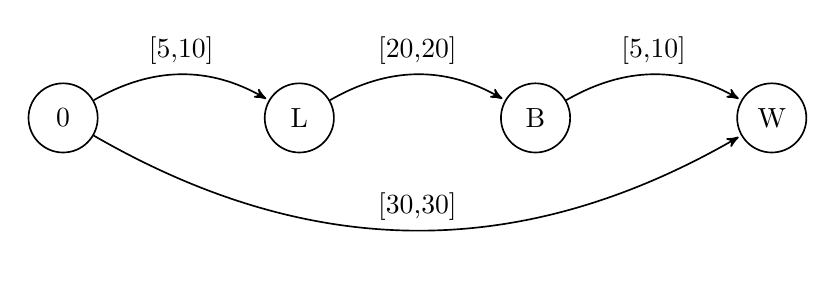
\begin{tikzpicture}[
	->,
	>=stealth',
	shorten >=1pt,
	auto,
	node distance=3cm,
     semithick
  ]

  \node[state] (1) 					{0};
  \node[state] (2) [right of=1] 		{L};
  \node[state] (3) [right of=2] 		{B};
  \node[state] (4) [right of=3] 		{W};

  \path (1) 	edge [bend left]    	node {[5,10]} 	(2)
            		edge [bend right] 	node {[30,30]} 	(4)
       	 (2) 	edge [bend left]		node {[20,20]} 	(3)
        	 (3) 	edge [bend left]     	node {[5,10]} 	(4);
        
\end{tikzpicture}

The goal of this graph is to associate each time point with a \emph{time window}, which is nothing more than an interval with a lower and an upper bound, in such a way that if each time point is associated with a value that lies within its time window, the schedule is consistent.

\subsubsection{Distance Graph}


\TODO{Bastiaan + Mick}
%		-Wat is een STN probleem (wat is het resultaat)
%		-Complexiteit
%		-Hoe los je het op


\subsubsection{Reduction to STN}


\TODO{Bastiaan + Mick}
%		-Het is dus geen goeie/volledige reductie :(
%		-Algemene/formele reductie Reductiedefinitie


\subsection{Resource}

\TODO{Bastiaan + Mick}
%		-Uitleggen huidige STN niet werkt (alleen temporal en niet resource feasable)
%		-Globale idee van resource leveling using PCP
%		-Algoritmw voor resource leveling (volgens ESTA en aan de hand van example)
%		-Algemeen en Formeel algoritme

\subsection{Final Schedule}

\TODO{Bastiaan + Mick}
%		-Hoe maak je van dat STN weer een schedule
%		-Hoe voldoet het schedule (aan alle constraints)


\newpage


\section{Conclusion}

\TODO{Roelf}



\newpage
\bibliographystyle{plainnat}
\bibliography{references}

\end{document}
